\documentclass[12pt]{article}
\setlength{\oddsidemargin}{0in}
\setlength{\evensidemargin}{0in}
\setlength{\textwidth}{6.5in}
\setlength{\parindent}{0in}
\setlength{\parskip}{\baselineskip}
\usepackage{amsmath,amsfonts,amssymb}
\usepackage{graphicx}
\usepackage[]{algorithmicx}
\usepackage{algpseudocode}


\usepackage[edges]{forest}
\usetikzlibrary{arrows.meta}
\usepackage{enumitem}
\usepackage{fancyvrb}
\usepackage{ wasysym }

\usepackage{fancyhdr}
\pagestyle{fancy}
\setlength{\headsep}{36pt}

\usepackage{hyperref}


\hypersetup{
    colorlinks=true,
    linkcolor=blue,
    filecolor=magenta,      
    urlcolor=blue,
}

\newcommand{\makenonemptybox}[2]{%
%\par\nobreak\vspace{\ht\strutbox}\noindent
\item[]
\fbox{% added -2\fboxrule to specified width to avoid overfull hboxes
% and removed the -2\fboxsep from height specification (image not updated)
% because in MWE 2cm is should be height of contents excluding sep and frame
\parbox[c][#1][t]{\dimexpr\linewidth-2\fboxsep-2\fboxrule}{
  \hrule width \hsize height 0pt
  #2
 }%
}%
\par\vspace{\ht\strutbox}
}
\makeatother

\begin{document}
\lhead{{\bf CSCI 3104, Algorithms \\ Homework 4 (100 pts)} }
\rhead{Name: \fbox{% Place your name here and delete the next time
\phantom{This is a really long name}} 
\\ ID: \fbox{ % Place your ID here and delete the next time
\phantom{This is a student ID}} 
\\ {\bf Escobedo \& Jahagirdar\\ Summer 2020, CU-Boulder}}
\renewcommand{\headrulewidth}{0.5pt}

\phantom{Test}

\begin{small}
\textit{Advice 1}:\ For every problem in this class, you must justify your answer:\ show how you arrived at it and why it is correct. If there are assumptions you need to make along the way, state those clearly.
%\vspace{-3mm} 

\textit{Advice 2}:\ Verbal reasoning is typically insufficient for full credit. Instead, write a logical argument, in the style of a mathematical proof.\\
%\vspace{-3mm} 

\textbf{Instructions for submitting your solution}:
\vspace{-5mm} 

\begin{itemize}
	\item The solutions \textbf{should be typed}, we cannot accept hand-written solutions. Here's a short intro to \href{http://ece.uprm.edu/~caceros/latex/introduction.pdf}{\textbf{Latex}.}
	 \item In this homework we denote the asymptomatic \textit{Big-O} notation by $\mathcal{O}$ and \textit{Small-O} notation is represented as $o$. 
	\item We recommend using online Latex editor \href{https://www.overleaf.com/}{\textbf{Overleaf}}. Download the \textbf{.tex} file from Canvas and upload it on overleaf to edit.
	%todo add link of gradescope
	\item You should submit your work through \href{https://www.gradescope.com}{\textbf{Gradescope}}  only.
	\item If you don't have an account on it, sign up for one using your CU email. You should have gotten an email to sign up. If your name based CU email doesn't work, try the identikey@colorado.edu version. 
	\item Gradescope will only accept \textbf{.pdf} files (except for code files that should be submitted separately on Canvas if a problem set has them) and \textbf{try to fit your work in the box provided}. 
	\item You cannot submit a pdf which has less pages than what we provided you as Gradescope won't allow it.
   
\end{itemize}
\vspace{-4mm} 
\end{small}

\hrulefill
\pagebreak

\subsection*{Piazza threads for hints and further discussion}
\begin{center}
    \begin{tabular}{|c|}
    \hline
    Piazza Threads \\ [0.5ex] 
    \hline \hline 
     \href{https://piazza.com/class/ka2roz7rb9m3j4?cid=50}{Question 1a}\\
     \href{https://piazza.com/class/ka2roz7rb9m3j4?cid=51}{Question 1b}\\
     \href{https://piazza.com/class/ka2roz7rb9m3j4?cid=52}{Question 1c}\\
     \href{https://piazza.com/class/ka2roz7rb9m3j4?cid=53}{Question 1d}\\
     \href{https://piazza.com/class/ka2roz7rb9m3j4?cid=54}{Question 1e}\\
     \href{https://piazza.com/class/ka2roz7rb9m3j4?cid=55}{Question 2}\\
     \href{https://piazza.com/class/ka2roz7rb9m3j4?cid=56}{Question 3}\\
    \hline
    \end{tabular}
\end{center}

\textbf{Recommended reading}: \\
\textbf{Dynamic Programming}: Chapter 15 complete 
\pagebreak

\begin{enumerate}
    
    \item (65 pts) The sequence $L_n$ of Lucas numbers is defined by the recurrence relation
	 $$L_n=L_{n-1}+L_{n-2}~~~~~~~~~~~~~~~~(1)$$ 
	 with seed values $L_0=2$ and $L_1=1$. 
	
	\begin{enumerate}[label=(\alph*)]
	

	\item \label{q:3:memfia}   (14 pts)   Consider the recursive top-down implementation of the recurrence (1) for calculating the $n$-th Lucas number $L_n$.  
	\begin{enumerate}
	\item (8 pts) Write down an algorithm for the recursive top-down implementation in pseudocode.  \\
	\makenonemptybox{3in}{
			\begin{algorithmic}[1]
			\Function{nLucas}{n}
			\State \If{n==0}{ \State \Return 2 }\EndIf
			\State \If{n==1}{ \State \Return 1 }\EndIf	
		\State	\Return $\Call{nLucas}{n-1} + \Call{nLucas}{n-2}$
		\end{algorithmic}
		
}

	\clearpage
    \item (2 pts) Draw the tree of function calls to calculate $L_5$. You can call your function $f$ in this diagram.\\
	\makenonemptybox{3.5in}{
		\begin{center}
		\begin{forest}
			for tree={
				align=center,
				font=\sffamily,
				edge+={thick, -{Stealth[]}},
				l sep'+=14pt,
				fork sep'=14pt,
			},
			forked edges,
			if level=0{
				tikz={\draw [thick] (.children first) -- (.children last);}
			}{},
			[$L_{5}$
			[$L_{4}$
			[$L_{3}$
			[$L_{2}$
			[$L_{1}$][$L_{0}$]
			][$L_{1}$]
			]
			[$L_{2}$
			[$L_{1}$][$L_{0}$]
			]
			][$L_{3}$
			[$L_{2}$
			[$L_{1}$][$L_{0}$]
			][$L_{1}$]
			]
			]
		\end{forest}
	\end{center}
	
}
	
	\item (4 pts) Write down the recurrence relation along with the base case for the running time $T(n)$ of the algorithm.\\
% 	and solve for it.
	\makenonemptybox{3in}{
Base Condition
T(0) = 2, T(1)=	1
\\
Recurrence Relation
T(n)= T(n-2) + T(n-1)
\\where T(n) is the running time 
}
		\\
	\item \label{q:3:memfib} (18 pts) Consider the dynamic programming approach ``top-down implementation with memoization'' that memoizes the intermediate Lucas numbers by storing them in an array $L[n]$. 
		
	\begin{enumerate}
	\item (10 pts) Write down an algorithm for the top-down implementation with memoization in pseudocode.  \\
	\makenonemptybox{5in}{
	\begin{algorithmic}[1]

		\Require{$L_{0}, L_{1}$} 

		\Ensure{$n^{th}$ Lucas Number}

		\Statex

		\Function{LucasTopDown}{n}
		\State \textit{$L[n]=-1$}
		\State \If{n==0}{ $L[n]=0$ }
		\State \ElsIf{n==1}{ $L[n]=1$ }
\State	\Else { L[n]=\Call{LucasTopDown}{n-1}+\Call{LucasTopDown}{n-2} }
\State \Return L[n] 
%\EndFunction
	\end{algorithmic}

}
	
	\clearpage
	\item (2.5 pts) Draw the tree of function calls to calculate $L_5$. You can call your function $f$ in this diagram.\\
	\makenonemptybox{3in}{
		\begin{center}
		
		\begin{forest}
			for tree={
				align=center,
				font=\sffamily,
				edge+={thick, -{Stealth[]}},
				l sep'+=13pt,
				fork sep'=13pt,
			},
			forked edges,
			if level=0{
				tikz={\draw [thick] (.children first) -- (.children last);}
			}{},
			[$L_{5}$
			[$L_{4}$
			[$L_{3}$
			[$L_{2}$
			[$L_{1}$][$L_{0}$]
			][$L_{1}$]
			]
			[$L_{2}$]
			][$L_{3}$]
			]
	\end{forest}
	\end{center}
}

	\item (2 pts) In order to find the value of $L_5$, you would fill the array $L$ in a certain order. Provide the order in which you will fill $L$ showing the values. \\
	\makenonemptybox{2in}{
		\begin{itemize}
		
			\item Lucas[5]=Lucas[4]+Lucas[3]
			
			\item Lucas[4]=Lucas[3]+Lucas[2]
			
			\item Lucas[3]=Lucas[2]+Lucas[1]
				\item Lucas[2]=Lucas[0]+ Lucas[1]
				\item Lucas[0]=2, Lucas[1]=1
		
		\end{itemize}
}
	
    \clearpage
	\item (4 pts) Determine and justify briefly the asymptotic running time $T(n)$ of the algorithm. \\
% 	Prove your claim is correct by induction on the contents of the array.
	\makenonemptybox{2in}{
Time Complexity is linear in time ie O(n).
As the previous computed values is already stored in memoization table. Lookup time : O(1) and for $n^{th}$ Lucas Number,it will have n-1 iterations.\\
Hence Time complexity :(n-1) $\times$ O(1) = O(n).	
}
	
	\end{enumerate}
	
	\item (16 pts) Consider the dynamic programming approach ``iterative bottom-up implementation'' that builds up directly to the final solution by filling the $L$ array in order. 	
	\begin{enumerate}
	\item (10 pts) Write down an algorithm for the iterative bottom-up implementation in pseudocode.  \\
    \makenonemptybox{4in}{
   % \begin{algorithm}
    	\begin{algorithmic}[1]

    		\Require{$L_{0}, L_{1}$} 

    		\Ensure{$n^{th}$ Lucas Number}

    		\Statex

    \Function{LucasBottomUp}{$n$}
    		\State $L[0]\gets 2$
    		\State $L[1]\gets 1$

    	
    		\State \For{$i \gets 2$ to $N$}

    		\State $L[i]=L[i-1]+L[i-2]$
    		\EndFor

    		 \State \Return {$L[n]$}
   % \EndFunction
    	\end{algorithmic}
%\end{algorithm}
}
    
    \item (2 pts) In order to find the value of $L_5$, you would fill the array $L$ in a certain order using this approach. Provide the order in which you will fill $L$ showing the values. \\
   \makenonemptybox{2.5in}{
   	\begin{itemize}
   	\item Lucas[0]=2, Lucas[1]=1
   	\item Lucas[2]=Lucas[0]+ Lucas[1]
   	  	\item Lucas[3]=Lucas[2]+Lucas[1]
   	  		\item Lucas[4]=Lucas[3]+Lucas[2]
   	  		 	\item Lucas[5]=Lucas[4]+Lucas[3]  	
\end{itemize}}
    
	\item (4 pts) Determine and justify briefly the time and space usage of the algorithm. \\
	\makenonemptybox{2in}{Time Complexity: O(n) as it will be having n iteration and each operation takes O(1).\\Space Complexity:O(n) as additional(or auxillary) array of size n is required for storing memoized values.}


	\end{enumerate}

	\clearpage
	\item (7 pts) If you only want to calculate $L_n$, you can have an iterative bottom-up implementation with $\Theta(1)$ space usage.  Write down an iterative algorithm with $\Theta(1)$ space usage in pseudocode for calculating $L_n$. There is no requirement for the runtime complexity of your algorithm. Justify your algorithm does have $\Theta(1)$ space usage.
    \makenonemptybox{6.5in}{
    	\begin{algorithmic}[1]

    	\Require{$L_{0}, L_{1}$} 

    	\Ensure{$n^{th}$ Lucas Number}

    	\Statex

    	\Function{LucasIterative}{$n$}
    	\State $a\gets 2$
    	\State $b\gets 1$

    	\STATE \If{n==0}
    	{
    		\Return a \;
    	}
    	\For{$i \gets 2$ to $N$}

    	\State { c = a + b} 

    	\State {a = b} 

    	\State {b = c} 
    	\EndFor

    	\State \Return {$b$}
    %	\EndFunction
    \end{algorithmic}

As no additional space in the form of array is required and each iteration takes O(1) space. Hence space complexity is O(1).
}
	
	
	\item (10 pts) In a table, list each of the four algorithms(as part of (a), (b), (c), (d)) as rows and in separate columns, provide each algorithm's asymptotic time and space requirements. Briefly discuss how these different approaches compare, and where the improvements come from.
	\makenonemptybox{6in}{

\vspace{2mm}
		\begin{tabular}{|c|c|c|}
			\hline
			\textbf{Question} & \textbf{Time Complexity} & \textbf{Space Complexity}\\

			\hline

			a & $2^{n}$ & N\\

			b & N & N\\

			c & N & N\\
			d&N&1\\
			\hline

		\end{tabular}
	
	
	\\
	Using top-down and iterative bottom up uses the concept of memoization, in which past values are stored.This prevents repetition of subproblem. Hence reduces time complexity from exponential to linear in 1.b and 1.c
	For the storing the previous computed values,memoization table in the form of array is required. 
}
	\end{enumerate}
	

    \clearpage
    
    \item {  (10 pts) Consider the following DP table for the Knapsack problem for the list $A = [(12, 9), (3, 6), (9, 3), (15, 12), (18, 9)] $ of (weight, value) pairs. \\
    The weight threshold $W = 30$.
    \begin{itemize}
        \item Fill in the values of the table.
        \item Draw the backward path consisting of backward edges and do not draw (or erase them) the edges that are not part of the optimal backward paths.
    \end{itemize}

    \begin{enumerate}[label=(\alph*)]
    \item (6 pts) Fill the table with the above requirements (You can also re-create this table in excel/sheet or on a piece of paper and add picture of the same).
    %\begin{table}
    \begin{center}
    \begin{tabular}{|c|c|c|c|c|c|c|c|c|c|c|c|c|c|}
    \hline
    Weight &  Value &  items\_considered & 0 & 1 & 2 & 3 & 4 & 5 & 6 & 7 & 8 & 9 & 10 \\ [0.5ex] 
    \hline \hline 
    - & - &  no items  & & & & & & & & & & & & 
    \hline
    12 & 9 & A[0..0] & & & & & & & & & & & & 
    \hline
    3 & 6 & A[0..1] & & & & & & & & & & & & 
    \hline
    9 & 3 & A[0..2] & & & & & & & & & & & & 
    \hline
    15 & 12 & A[0..3] & & & & & & & & & & & & 
    \hline
    18 & 9 & A[0..4] & & & & & & & & & & & & 
    \hline
    \end{tabular} \\ \\
    \end{center}
%\end{table}


\begin{figure}[h!]
	\begin{center}
		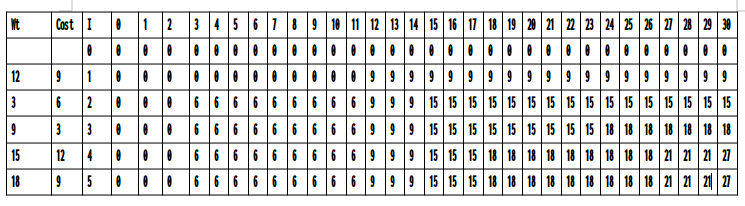
\includegraphics[scale=0.75]{HW2.png}
	\end{center}
\end{figure}   

\end{enumerate}
    \item (2 pts) Which cell has the optimal value and what is the optimal value for the given problem?
    \makenonemptybox{3in}{
    	Cell containing weight 15 has optimal value, ie Item 3.\\ Optimal Value: 27 units
    }
    
    
    \item (2 pts) List out the optimal subset and provide it's weight and value.
    \makenonemptybox{3in}{
Optimal Subset : (Weight, Value)\\
(3,6),(15,12) ,(12,9).
\\Optimal Value:27 units  
}
  %  \end{enumerate}}
    
    \clearpage 
    
    \item{ (25 pts) Given an array of $n$ size, the task is to find the longest subsequence such that the \textbf{absolute difference} between two adjacent values in the sequence is odd and less than or equal to 5. i.e the \textbf{absolute difference} between the adjacent elements is one of the values from the set $\{1, 3, 5\}$ \\
   For the definition of subsequence click \href{https://www.geeksforgeeks.org/subarraysubstring-vs-subsequence-and-programs-to-generate-them/}{here}\\ 


    \textbf{Example 1}:\\
    \textbf{Input}: $\{10, 30, 5, 8, 27, 1, 4, 9, 14, 17\}$\\
    \textbf{output}: 6\\
    \textbf{Explanation}: Here the longest sequence satisfying the above condition will be \\
    $\{10, 5, 8, 9, 14, 17\}$ having a size of 6\\ \\
    
    \textbf{Example 2}:\\
    \textbf{Input}: $\{10, 30, 6, 9, 27, 22, 20, 19\}$\\
    \textbf{output}: 4\\
    \textbf{Explanation}: There are several sequences of length 4 one such sequence is \\
    $\{30, 27, 22, 19\}$ having a size	 of 4\\ \\
    
    \begin{enumerate}[label=(\alph*)]
    \item{ (5 pts)
    State the base case and recursive relation that can be used to solve the above problem using dynamic programming.  
    }
    \makenonemptybox{2in}{
    	LCS(A[],i) = \begin{cases}
    	 1, & \text{if } i$\leq$0 \\
    max(1,max (1,	1+LCS(A[],i))), &  i>0,$diff=\{1,3,5\}$\\

    \end{cases}\\
where A[.] is the array containing element and i is the index of array
}

    \clearpage
    \item{ (10 pts)
    Write down well commented pseudo-code or paste real code to solve the above problem. 
    }
    \makenonemptybox{6.5in}{
    	\begin{algorithmic}[1]
 	\Function{LCSDiff}{A[], idx}
 
 	\State \If{idx==0}{ \Return 1 \;}
 		\Comment{Only one subsequence ends at first index, the number itself}
 
 	\State $ans\gets 1$
 		\Comment{As answer keeps on changing, so initialize to idx value}
 
 	\State \For{$i \gets idx-1$ to $0$}
 		\Comment{Comparing the first element with remaining element and checking if difference is 1 or 3 or 5}
 	\State \If{abs(A[idx]-A[i])$\leq$5 and (A[idx]-A[i])\%2$\neq$0 }
 	{\newline $ans \gets max(1,max(ans,1+\Call{LCSDiff}{A[],i}))$}
 	\EndIf
 	\EndFor
 	
 \State \Return  $ans$ \Comment{Return the length of answer}
 \EndFunction
\end{algorithmic}


}
    
    \clearpage
    \item{ (5 pts)
    Discuss the space and runtime complexity of the code, providing necessary justification. 
    }
    \makenonemptybox{3in}{$O(N)$ for iterating and comparison of difference with adjacent element is less than 5 and is odd. $O(N)$ for returning the maxlength of such subsequence.Time complexity : $O(N) \times O(N)=O(n^{2})$,  
    	\\Space Complexity: O(N), as auxillary array is used for storing the result. 
    }
    
    \item{ (5 pts)
     Show how you can modify your pseudo-code or real code to return an optimal subsequence (if the problem has multiple optimal subsequences as part of it's solution, it is sufficient to return any one of those). 
    }
    \makenonemptybox{3in}
    {
    	Instead of 2 for loops, we can use Hashmap for searching and storing the required answer in the hashmap. This will reduce time complexity to $O(N)$, as n times for searching and n times for storing required answer into hashmap.\\If there are multiple optimal substructure,then storing the answer with the index pair will give us the answer.
    
	}
    \end{enumerate}
    
    }
    
    \item{\itshape \textbf{Extra Credit (5\% of total homework grade)}
    For this extra credit question, please refer the leetcode link provided below or click \href{https://leetcode.com/problems/regular-expression-matching/}{here}. Multiple solutions exist to this question ranging from brute force to the most optimal one. Points will be provided based on Time and Space Complexities relative to that of the most optimal solution.

    Please provide your solution with proper comments which carries points as well.}
    
   \url{https://leetcode.com/problems/regular-expression-matching/}
   
 

    % Paste your code in the verbatim tag below
\begin{verbatim}
Replace this text with your source code inside of the .tex document
\end{verbatim}	
    
    
	
\end{enumerate}


\end{document}


